\begin{figure}[htbp]
			\centering
			\resizebox{\textwidth}{!}{%
				\begin{tikzpicture}[scale=0.95,>=latex,
					trave/.style={line width=1.4pt},
					forza/.style={black, line width=0.8pt},
					diagT/.style={black, line width=0.6pt},
					diagM/.style={black, line width=0.6pt},
					hatch/.style={gray!50, line width=0.3pt},
					quota/.style={black, line width=0.4pt},
					fibre/.style={gray!70, line width=0.3pt},
					]
					\def\tw{0.15}\def\thR{0.28}\def\rn{0.06}
					\def\rw{0.05}\def\bw{0.09}\def\gw{0.22}\def\hh{0.10}
					\def\Lell{4}\pgfmathsetmacro{\xMid}{0.5*\Lell}
					\def\yqi{-0.80}\def\ylab{-1.35}
					\def\rCoppia{0.25}\def\Lwing{0.12}\def\AoffX{0.20}\def\BoffX{0.20}
					% ── trave + cerniera A + carrello B + perni + etichette ──
					\def\vincoli{%
						\draw[thick] (0,0) -- (-\tw,-\thR) -- (\tw,-\thR) -- cycle;
						\draw[thick] (-\gw,-\thR) -- (\gw,-\thR);
						\foreach \x in {-0.16,-0.08,0,0.08,0.16}\draw[thin] (\x,-\thR) -- ++(-0.07,-\hh);
						\draw[thick] (\Lell,0) -- (\Lell-\tw,-\thR) -- (\Lell+\tw,-\thR) -- cycle;
						\draw[thick] (\Lell-\bw,-\thR-\rw-0.01) circle (\rw);
						\draw[thick] (\Lell+\bw,-\thR-\rw-0.01) circle (\rw);
						\draw[thick] (\Lell-\gw,-\thR-2*\rw-0.04) -- (\Lell+\gw,-\thR-2*\rw-0.04);
						\foreach \x in {-0.16,-0.08,0,0.08,0.16}\draw[thin] (\Lell+\x,-\thR-2*\rw-0.04) -- ++(-0.07,-\hh);
						\draw[thick, fill=white] (0,0) circle (\rn);
						\draw[thick, fill=white] (\Lell,0) circle (\rn);
						\node[above left=-2pt, font=\small] at (0,0) {$A$};
						\node[above right=-2pt, font=\small] at (\Lell,0) {$B$};}
					% ── coppia antioraria in A ──
					\def\coppiaA#1{%
						\draw[forza] (\AoffX,-\rCoppia) arc[start angle=-90, end angle=90, radius=\rCoppia];
						\draw[forza] (\AoffX,\rCoppia) -- ({\AoffX+\Lwing*cos(25)},{\rCoppia+\Lwing*sin(25)});
						\draw[forza] (\AoffX,\rCoppia) -- ({\AoffX+\Lwing*cos(-25)},{\rCoppia+\Lwing*sin(-25)});
						\node[right, font=\footnotesize] at (\AoffX+\rCoppia+0.02,0.16) {#1};}
					
					% (a) schema: sola coppia chi_1=1 in A
					\begin{scope}[xshift=0cm]
						\draw[trave] (0,0) -- (\Lell,0);
						\draw[fibre, dashed] (0,-0.1) -- (\Lell,-0.1);
						\vincoli
						\coppiaA{$\chi_1=1$}
						\node[font=\small] at (\xMid,\ylab/2) {(a)};
					\end{scope}
					% (b) T_1 = 1/l uniforme
					\begin{scope}[xshift=5.5cm]
						\draw[trave] (0,0) -- (\Lell,0);
						\def\Tf{0.45}
						\foreach \x in {0.10,0.30,...,3.90}\draw[hatch] (\x,0) -- (\x,\Tf);
						\draw[diagT] (0,0) -- (0,\Tf) -- (\Lell,\Tf) -- (\Lell,0);
						\vincoli
						\node[font=\small] at (\xMid,{0.5*\Tf}) {$\boldsymbol{\oplus}$};
						\node[font=\small] at (3.75,{\Tf+0.30}) {$\tfrac{1}{\ell}$};
						\draw[quota, ->] (3.55,{\Tf+0.20}) -- (3.3,{0.5*\Tf});
						
						\node[font=\small] at (\xMid,\ylab/2) {(b)};
					\end{scope}
					% (c) M_1: da -1 in A (sopra l'asse) a 0 in B
					\begin{scope}[xshift=11.0cm]
						\draw[trave] (0,0) -- (\Lell,0);
						\def\hM{0.7}
						\foreach \x in {0.10,0.30,...,3.90}{\pgfmathsetmacro{\h}{\hM*(1-\x/\Lell)}\draw[hatch] (\x,0)--(\x,\h);}
						\draw[diagM] (0,0) -- (0,\hM) -- (\Lell,0);
						\vincoli
						\node[left, font=\small] at (0,\hM+0.02) {$1$};
						\node[font=\small] at (\xMid,\ylab/2) {(c)};
					\end{scope}
				\end{tikzpicture}
			}
			\caption{Problema ``1'': coppia unitaria in $A$ (a);
				taglio $T_1$ (b); momento $M_1$ (c).}
			\label{fig:stat_iper_trasv_01-p1}
		\end{figure}
